% For si figures and text

% \renewcommand\thefigure{D\arabic{figure}} % Rename figures with Appendix index   
% \renewcommand\thetable{D\arabic{table}}   
% \setcounter{figure}{0}    
% \setcounter{table}{0}

\renewcommand\thefigure{A\arabic{figure}} % Rename figures with Appendix index  -Weiwei He
\renewcommand\thetable{A\arabic{table}}  
\renewcommand\theequation{A\arabic{equation}}
\setcounter{figure}{0}    
\setcounter{table}{0}
\setcounter{equation}{0}

\newappendix{Appendix A: Supplementary Material For Chapter ~\ref{ch_chapter1}}

\subsection*{Bridging Concepts and Discoveries}

\subsubsection*{From Theory to Application}

\begin{table}
\centering
\caption{Data sheet}
\label{tbl:ch1si-table}
\begin{threeparttable}
\begin{tabular}{lcccccc}
\toprule
{} &   \specialcell{Column 1}  & \specialcell{Column 2} & \specialcell{Column 3} & \specialcell{Column 4} \\
\midrule
A &  B  & C &  D & E\\
A  &  B & C & D & E \\
A  &  B & C & D & E \\
A  &  B & C & D & E \\
A  &  B & C & D & E \\
A  &  B & C & D & E \\
A  &  B & C & D & E \\
\bottomrule
\end{tabular}
\begin{tablenotes}
\small
\item Notes Notes Notes Notes Notes Notes Notes Notes Notes
\end{tablenotes}
\end{threeparttable}
\end{table}

\newpage
\clearpage

\subsection*{Supporting Figures}
\begin{figure}[ht]
\centering
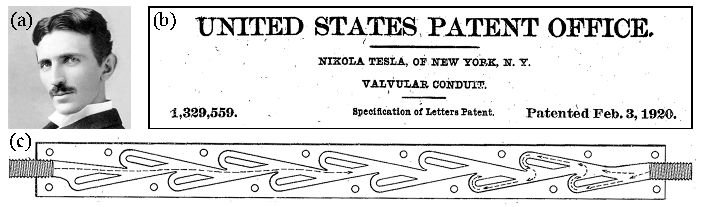
\includegraphics[width=16.5cm]{figures/ch_chapter1/fig1.pdf}\vspace{-0.2cm}
\caption{(a) The genius Nikola Tesla (b) His patent (c) Tesla's channel }
\label{fig:ch1si-patent}
\end{figure}